\chapter{Das EVM8168-Entwicklungsboard}
\label{ch:board}
\rm

F�r die in den folgenden Kapiteln beschriebenen Arbeitsschritte zur Optimierung und Analyse des Programmes wurde ein EVM8168-Entwicklungsboard verwendet, welches von der Firma Texas Instruments in Zusammenarbeit mit der Firma Spectrum Digital entwickelt wurde.
Dieses Board kann mit Hilfe eines DM816x (DaVinci\texttrademark) ARM-Prozessors entweder selber Programme ausf�hren oder es k�nnen auch die beiden ARM-Prozessoren C6A816x (Integra\texttrademark) oder AM389x (Sitara\texttrademark) emuliert werden. 


\section{Aufbau des EVM8168} \label{sec:evm816}
Wie in \cite{spec} beschrieben bietet das EVM816x-Entwicklungsboard eine Standalone-Plattform um Programme f�r DaVinci\texttrademark, Integra\texttrademark~oder Sitara\texttrademark~Prozessoren der Firma Texas Instruments zu entwickeln und zu debuggen. Hierf�r sind neben dem DaVinci\texttrademark~noch weitere On-Board Peripherie auf dem Board aufgebracht, die im folgenden teilweise n�her erkl�rt werden sollen.
Das EVM8168-Board hat unter anderem folgende Komponenten integriert:

\begin{itemize}
	\item DM816x- (DaVinci\texttrademark-)ARMprozessor (\textbf{Kapitel~\ref{sec:davinci}}) mit NEON-Einheit (\textbf{Kapitel~\ref{subsec:neon}}) und DSP (\textbf{Kapitel~\ref{subsec:dsp}})
	\item 1 GB DDR3-RAM
	\item AC31061-Audiochip
	\item Gigabit Ethernet
	\item HDMI
	\item VGA
	\item USB

\end{itemize}

\textbf{Abbildung~\ref{fig:top_ti816x_evm}} zeigt eine Draufsicht auf das Entwicklungsboard und die unterhalb dessen angebrachte Daughtercard mit weiteren Anschlussm�glichkeiten.

\begin{figure}[htbp]
	\centering
		\includegraphics[scale=0.4]{../Pictures/top_ti816x_evm.png}
	\caption{Draufsicht auf das EVM8168}
	\label{fig:top_ti816x_evm}
\end{figure}



\section{Der DaVinci\texttrademark}\label{sec:davinci}
Bei dem auf dem EVM816x verwendeten ARM-Prozessor DM816x handelt es sich um einen eigentlich f�r die Videoprozessierung optimierten Prozessor der DaVinci\texttrademark-Familie von Texas Instruments.\\
Der DM816x ist ein heterogener Prozessor, der mehreren Subsystemen und Koprozessoren besteht.
Genauer gibt des folgende Subsysteme:

\begin{itemize}
\item ARM Subsystem mit einem Cortex-A8 der Firma ARM (\textbf{\ref{subsec:a8}})
\item DSP Subsystem mit einem C674x VLIW DSP der Firma Texas Instruments (\textbf{\ref{subsec:dsp}})
\item SGX530 3D Grafik Engine
\item 512kb On-Chip RAM
\item High-Definition Video Image Coprozessoren (HDVICP2)
\item Media Controller
\item HD Video Processing Subsysstem (HDVPSS)
\item System Control
\item Peripherie
\end{itemize} 

All diese Subsysteme und Coprozessoren sind durch eine gemeinsame System Interconnection miteinander verbunden. \textbf{Abbildung \ref{fig:dm8168}} zeigt das funtionale Blockdiagram des DM816x \cite{evm8168}.\\
%
\begin{figure}[htbp]
	\centering
		\includegraphics[width=1\textwidth]{../Pictures/dm8168.pdf}
	\caption{Funtionales Blockdiagramm des DM816x\cite{evm8168}}
	\label{fig:dm8168}
\end{figure}
%

\subsection{ARM Cortex-A8}\label{subsec:a8}

Der erste Prozessor aus der heterogenen Prozessorarchitektur des DM8168 der vorgestellt werden soll, ist ein Cortex-A8 der Firma ARM. Hierbei handelt des sich um einen General-Purpose Prozessor im RISC Design. Er besteht im wesentlichen aus 7 Komponenten (vgl. \textbf{Abbildung \ref{fig:a8}}):

\begin{itemize}
	\item Instruction Fetch
	\item Instruction Decode
	\item Instruction Execute
	\item Load/Store
	\item L2 Cache
	\item NEON-Coprozessor (\textbf{\ref{subsubsec:neon}})
	\item ETM
\end{itemize}
%
\begin{figure}[h]
	\centering
		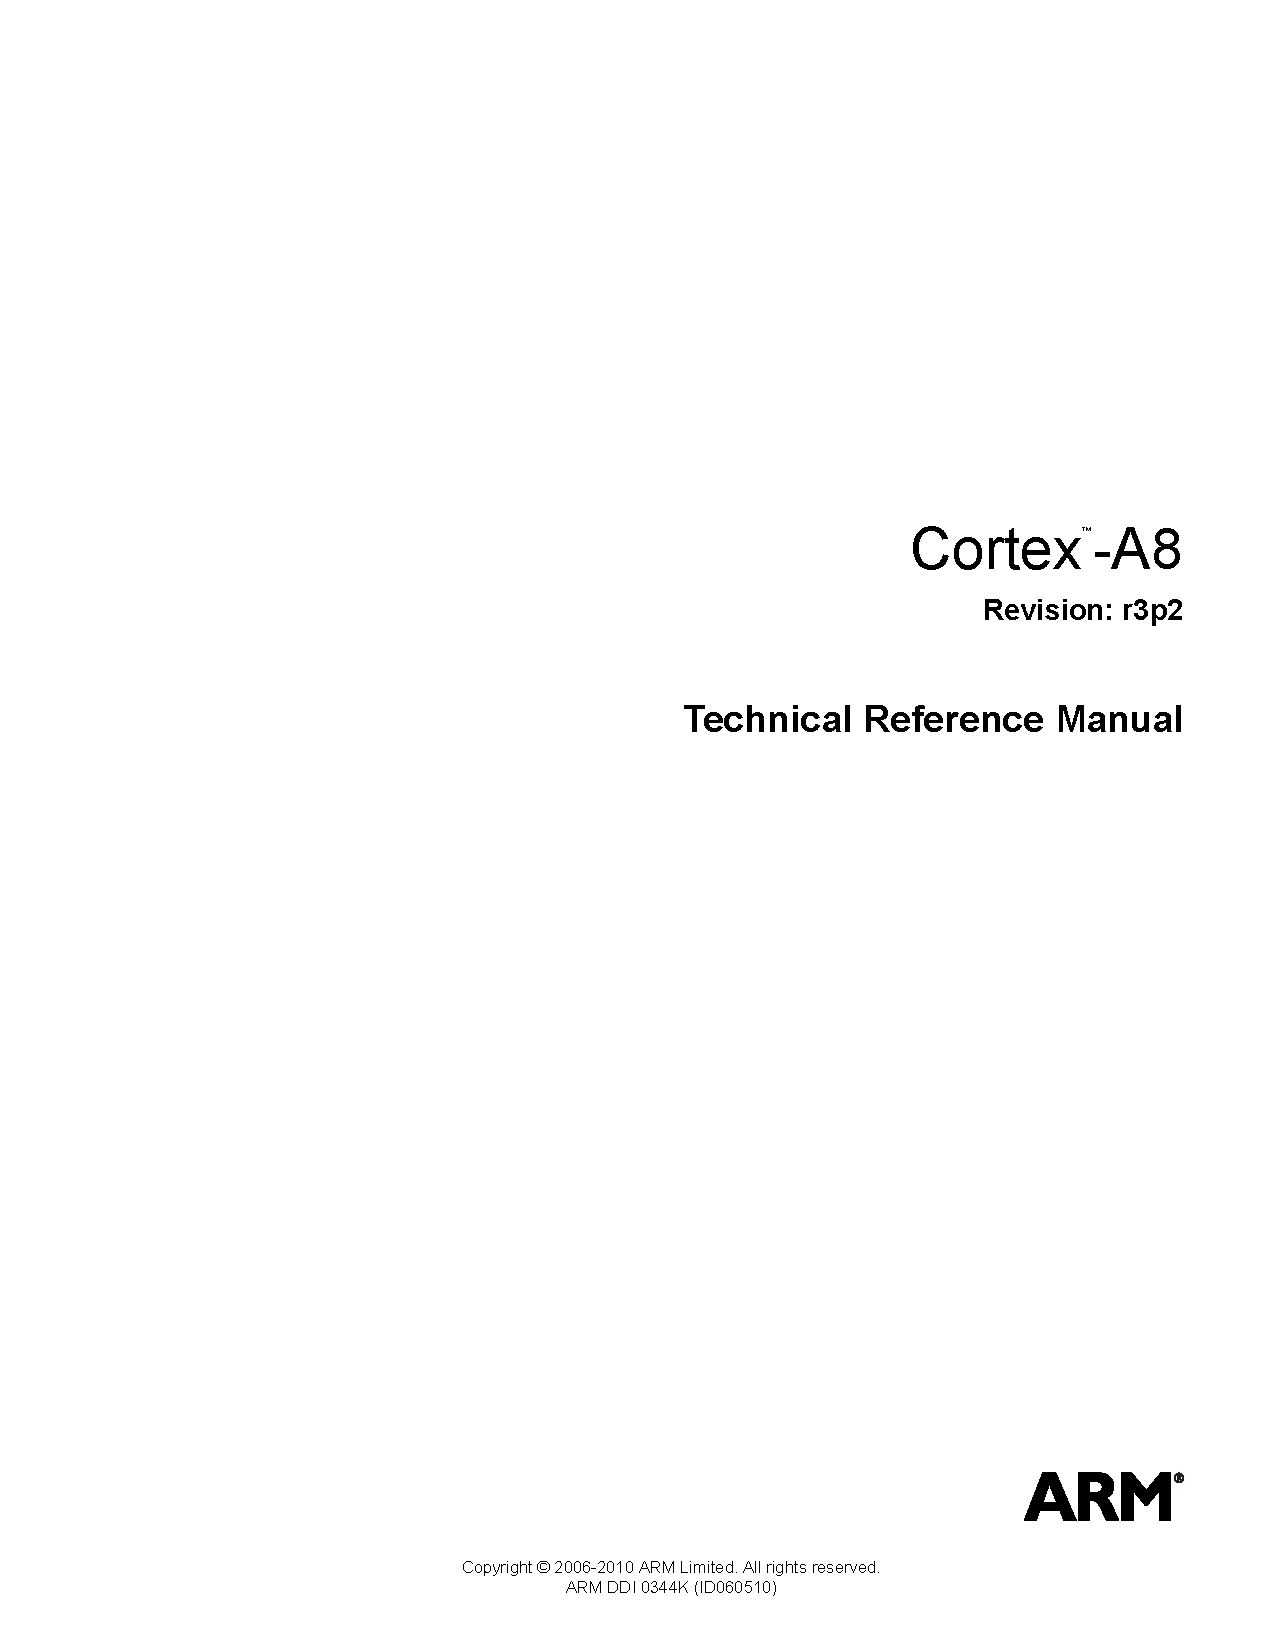
\includegraphics[width=1\textwidth]{../Pictures/cortexa8.pdf}
	\caption{Cortex-A8 Blockdiagramm\cite{cortexa8}}
	\label{fig:a8}
\end{figure} 
%
Wie auf in der Abbildung eventuell etwas schwer zu sehen ist, stellt der Cortex-A8 einen heterogenen Dualcore-Prozessor dar. Dieser besteht aus einem ARMv7 Prozessorkern (\textbf{\ref{subsubsec:armv7}}) und einem NEON-Coprozessor (\textbf{\ref{subsubsec:neon}}).\\
Diese beiden Prozessoren teilen sich Instruction Fetch, Instruction Decode, Instruction Execute, Load/Store und L2 Cache \cite{cortexa8}.

\subsubsection{ARMv7-A Prozessorkern}\label{subsubsec:armv7}
Der ARMv7-A Prozessorkern ist f�r die Ausf�hrung von Integeroperationen zust�ndig. Diese werden in einer dreistufigen Pipeline ausgef�hrt, die aus Fetch, Decode und Execute besteht.\\
In der Fetch-Phase werden ben�tigte Befehle aus dem L1-Instruction-Cache geladen, der sich in der Instruction Fetch-Einheit befinden (vgl. \textbf{Abbildung \ref{fig:a8}}).\\
Diese Instruktionen werden in einen Buffer geladen, der im n�chsten Schritt von der Instruction Decode-Einheit ausgelesen und decodiert wird, au�erdem wird in der Decode-Phase die Ausf�hrungsreihenfolge der geladenen Befehle festgelegt. Diese Reihenfolge h�ngt unter anderem von den Registern und Takten ab, die f�r die Ausf�hrung ben�tigt werden (eine �bersicht der Intruktionen wird in \textbf{\ref{ph:a8inst}} gegeben).\\
In der Execute-Phase werden anschlie�end die Befehle an die entsprechenden Funktionseinheiten weitergeleitet.\\
Wie schon erw�hnt ist dieser Prozessorkern auf Integeroperationen ausgelegt, wird aber bei der Kompilierung eines Programms f�r den Cortex-A8 dem Compiler nicht die Benutzung einer Floating Point-Einheit vorgeschrieben (vgl. \textbf{Kapitel \ref{subsubsec:neon}}) werden auch entsprechende Befehle auf den Integeroperationen des ARMv7-A Prozessorkerns approximiert, was zu langen Ausf�hrungszeiten f�hren kann.  
\paragraph{Instruktionssatz}\label{ph:a8inst}$\;$ \\
\subsubsection{Der NEON-Coprozessor}\label{subsubsec:neon}
\paragraph{VFPv3-Einheit}$\;$ \\
\paragraph{NEON-SIMD-Einheit}$\;$ \\
\paragraph{Ansteuerungsm�klichkeiten}$\;$ \\
\subparagraph{Compiler}$\;$ \\
\subparagraph{C-Code}$\;$ \\
\subparagraph{Intrinsics}$\;$ \\
\subparagraph{Assembler}$\;$ \\
\subsection{Der C674x-DSP-Prozessor}\label{subsec:dsp}

Der C674x ist ein Floating-Point VLIW DSP mit 64 General-Purpose Registern mit je 32-Bit. Er besitzt sechs ALU Funktionseinheiten mit 32 und 40 Bit. Er unterst�tzt 32-Bit Floating Point Integer mit IEEE Single Precision (SP 32-Bit) und IEEE Double Precision (DP 64-Bit). Auf diesen schafft er bis zu vier SP Adds pro Takt und vier DP Adds alle zwei Takte, des weiteren kann er bis zu zwei Floating-Point approximierte reziproke oder quadratische Wurzeln pro Takt in SP oder DP berechnen.\\
Au�erdem besitzt er zwei Multiplizierer, entweder gemischt pr�zise Floating-Point oder Fixed-Point Integer berechnen k�nnen. Im Floating-Point-Modus schaffen diese folgende Berechnungen in den angegebenen Takten:

\begin{itemize}
	\item $2~SP \times SP~\rightarrow~ SP~pro~Takt$
	\item $2~SP \times SP~\rightarrow~ DP~pro~zwei~Takte$
	\item $2~SP \times DP~\rightarrow~ DP~pro~drei~Takte$
	\item $2~DP \times DP~\rightarrow~ DP~pro~vier~Takte$
\end{itemize}

Im Fixed-Point-Modus sind zwei 32x32, vier 16x16 oder acht 8x8 Multiplizierungen pro Takt m�glich.\\
Die Speicherarchitektur des C674x besteht aus zwei Ebenen, auf der Ersten sind 32K-Byte L1P und L1D RAM und Cache, auf der Zweiten 256K-Byte L2 RAM und Caches.\\
In der hier vorliegenden Architektur fungiert der DSP als Slave-Prozessor\cite{evm8168}.\linebreak
%
\begin{figure}[htbp]
	\centering
		\includegraphics[width=0.65\textwidth]{../Pictures/DSPBlock.pdf}
	\caption{Blockdiagramm des C764x\cite{evm8168}}
	\label{fig:bddsp}
\end{figure}
%
Wie man dem Blockdiagramm in \textbf{Abbildung \ref{fig:bddsp}} entnehmen kann, besitzt der C674x zwei Register, die parallel Operationen ausf�hren k�nnen. Jedes dieser Register besteht hierbei aus vier Funktionseinheiten, die mit .M, .L, .D und .S bezeichnet sind. Diese Funktionseinheiten haben die Eigenschaft, dass jede von ihnen eine Operation pro Takt ausf�hren kann, diese also auch parallel ausgef�hrt werden k�nnen. Den einzelnen Einheiten sind hierbei bestimmte Operationen zugeordnet. Die einzelnen Funktionseinheiten beinhalten folgende Operationen:

\begin{itemize}
	\item .D behandelt Lade- und Speicheroperationen
	\item .S behandelt Shift-, Sprung- und Vergleichsoperationen
	\item .M behandelt Multiplikationsoperationen
	\item .L behandelt logische und arithmetische Operationen 
\end{itemize}

Somit kommen wir auf 8 Funktionseinheiten, die parallel pro Takt eine Operation durch f�hren k�nnen. Je nachdem zu welchem Register sie zugeordnet sind werden sie entweder mit einer 1 oder mit einer 2 bezeichnet, nimmt man also zum Beispiel die D Funktionseinheit des Registers A, wird diese mit .D1 bezeichnet. In \textbf{Abbildung \ref{fig:reg}} ist dieses nochmals verdeutlicht.
%
\begin{figure}[h]
	\centering
		\includegraphics[scale=0.80]{../Pictures/Register.pdf}
	\caption{Registerarchitektur des C764x\cite{sprabf2}}
	\label{fig:reg}
\end{figure} 

\subsubsection{Hardware}
\paragraph{Registerarchitektur}$\;$ \\
\paragraph{Instruktionssatz}$\;$ \\
\paragraph{Pipelining auf dem C674x}$\;$ \\
\subsubsection{Compileroptimierungsstufen}
\subsubsection{Beispielverarbeitung des C674x}
\paragraph{Beispiel der Compileroptimierung}$\;$ \\
\paragraph{Beispiel des Software-Pipelinings (SPLOOP)}$\;$ \\
\subsubsection{Optimierte Bibliotheken f�r den C674x}